\documentclass{article}
\usepackage{graphicx}
\usepackage[sharp]{easylist}
\graphicspath{ {images/} }
\begin{document}
\fbox{\parbox{10cm}{\centering\Huge Product Specification}}
\\\\\\\\
\LARGE
Application Objective
\\
\normalsize
\\
The objective of this application is to make the extraordinary world of chess more accessible
to the people. No longer do you have to bring a big robust wooden board. You just have to
pick up your computer and start playing. Not only can you play by yourself but you can also play
against our advanced AI on the level that you prefer. With the magical and outstanding graphics
of our app, the game of chess will be more colourful and packed with mind blowing effects.
\\

\LARGE\noindent
System Requirement
\normalsize
\begin{easylist}[itemize]
    # Supported Platforms 
    ## Windows 10 or above
    ## Mac OSX High Sierra or above
    ## Ubuntu Linux
    # Hardware requirements:
    ## Processor: 32-bits or greater
    ## At least 512 MB RAM
    # Software Requirements:
    ## JAVA SE 8 or above
    # User requirements:
    ## Will work
    ## Should be able to play chess
\end{easylist}
\LARGE\noindent
\\
User Stories
\normalsize
\\
As a chess player, i expect the chess pieces to behave like they do in regular chess.

\noindent
As a user, i expect the game to easily be understandable

\noindent
As a user, i expect the game to look visually pleasing

\noindent
As a user, i expect the game to have simple controls

\noindent
As a user, i expect to be able to play this on my computer

\noindent
As a user, i expect the application to be responsive

\noindent
As a user, i expect the application to not crash

\LARGE
\newpage
\hspace*{+2,5cm} 
User Case Diagram
\\\\
\hspace*{-2cm}  
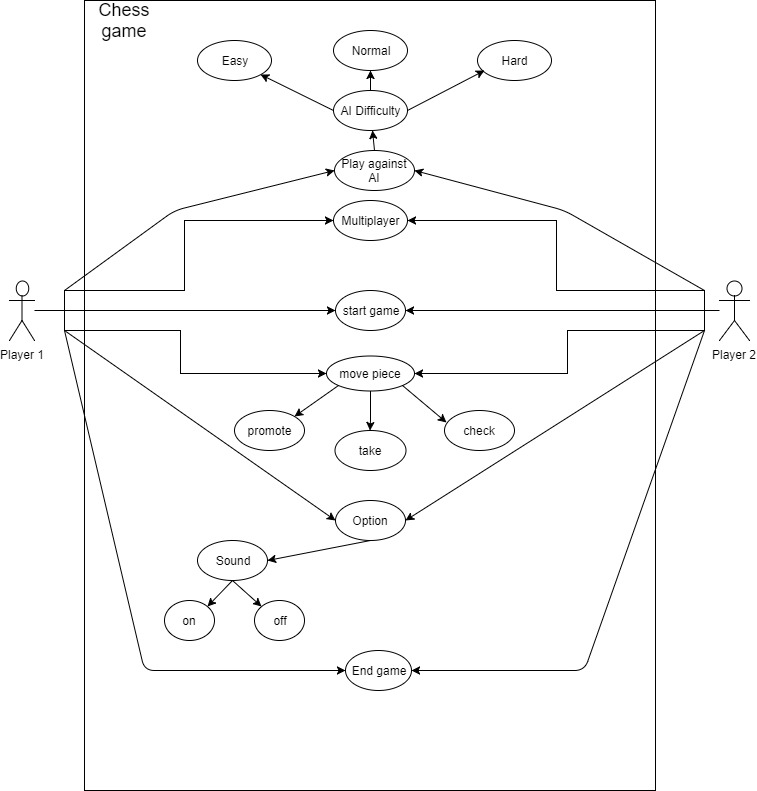
\includegraphics[scale=0.60]{usercasediagram}
\newpage
\noindent
\hspace*{+2,5cm} 
Class Case Diagram
\\\\\\
\hspace*{-4,5cm}  
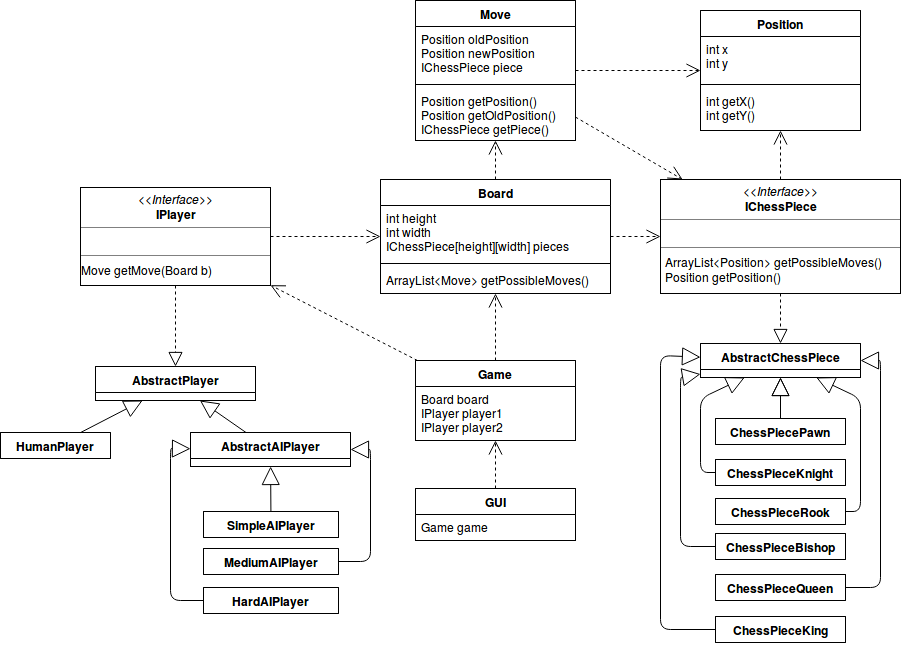
\includegraphics[scale=0.6]{classdiagram2}

\normalsize
\newpage
\section{Fully dressed use case \#1: Move a piece}

\paragraph{Use case name:} Move a piece

\paragraph{Scope:} Chess application gameplay

\paragraph{Level:} User goal

\paragraph{Primary actor:} Current player

\paragraph{Stakeholders and interests:}\mbox{}\\
- \textbf{Current player:} Wants to move a piece to a different square\\
- \textbf{Chess application:} Must restrict movement to a valid square\\
- \textbf{Opponent player:} Wants to be in a good position for their next move

\paragraph{Preconditions:} It's current player's turn to move. Previous moves have been logged. Previous moves have been valid.

\paragraph{Success guarantee (postconditions):} Exactly one of current player's pieces is in a different position. The move has been recorded. The recorded move was valid. It's opponent player's turn to move, or the game is over.
\paragraph{Main success scenario:}\mbox{}\\
1. Current player selects piece to move\\
2. Chess application indicates possible squares the player can move to\\
3. Current player selects one of the highlighted squares\\
4. Chess application validates move\\
5. Chess application performs move\\
6. Chess application checks for promotion\\
7. Chess application logs move\\
8. Chess application checks if the move resulted in check\\
9. Chess application displays the result\\
10. Chess application changes turn from current player to opponent player

\paragraph{Extensions:}\mbox{}\\
$*$a. At any time, current player may exit the game\\
\indent1. Chess application aborts current game\\
\indent2. On next startup, chess application displays an option to continue previous game\\
\indent\indent$*$a.2a. The player selects to continue the game\\
\indent\indent\indent1. The game is resumed from the start of the aborted turn\\
\indent\indent$*$a.2b. The player starts a new game\\
\indent\indent\indent1. The aborted game is discarded\\
\newpage
$*$b. At any time during their turn, the player may resign the game\\
\indent1. Chess application asks for confirmation\\
\indent\indent$*$b.1a. Current player confirms resignation\\
\indent\indent\indent1. Chess application records resignation\\
\indent\indent\indent2. Chess application ends current game with opponent player as the victor\\
\indent\indent\indent3. Chess application performs player ranking calculations\\
\indent\indent\indent4. Chess application displays the information that the player has resigned\\
\indent\indent\indent5. Current player exits the game\\
\indent\indent$*$b.1b. Current player cancels resignation\\
\indent\indent\indent1. Resume turn from last step\\
1a. Current player selects one of opponent player's pieces, or a square with no piece on it\\
\indent1. Chess application ignores the input\\
1b. Current player selects a piece which cannot move under the current conditions\\
\indent1. Chess application displays a notice saying the piece cannot move\\
\indent\indent1b.1a. Current player deselects piece\\
\indent\indent\indent1. Resume turn from step 1\\
\indent\indent1b.1b. Current player selects a different piece which cannot move\\
\indent\indent\indent1. Repeat step 1b\\
\indent\indent1b.1b. Current player selects a different piece which can move\\
\indent\indent\indent1. Resume turn from step 2\\
3a. Current player selects a square which is not indicated\\
\indent1. Chess application ignores the input\\
3b. Current player selects a different piece\\
\indent1. Resume turn from step 1 or any step 1 extension as appropriate\\
4a. The move is invalid (should not happen under normal circumstances)\\
\indent1. Chess application displays an error message\\
\indent2. Chess application sends anonymous error report to developers\\
\indent3. Resume turn from step 1\\
5a. The move was to an empty square\\
\indent1. Chess application updates position of moved piece on board\\
\indent2. Resume turn from step 6\\
5b. The move was to a square containing an opponent player's piece\\
\indent1. Chess application removes opponent player's piece from board\\
\indent2. Chess application updates position of moved piece on board\\
\indent3. Resume turn from step 6\\
6a. The move resulted in a promotion\\
\indent1. Chess application replaces pawn with queen\\
8a. The move results in check\\
\indent1. Chess application shows notice that opponent player is in check\\
8b. The move results in check mate\\
\indent1. Chess application shows notice that opponent player is in check mate\\
\indent2. Chess application ends current game with current player as the victor\\
\indent3. Chess application performs player ranking calculations\\
10a. The game has ended\\
\indent1. Chess application does not start opponent player's turn\\
\indent2. Chess application displays option to exit the game\\

\paragraph{Special requirements:}\mbox{}\\
- Mouse or keyboard input devices for player input\\
- Display screen for output\\
- Host computer needs a graphical user interface

\paragraph{Technology and data variations list:}\mbox{}\\
1a. Piece selection using mouse input\\
1b. Piece selection using keyboard input\\
3a. New position selection using mouse input\\
3b. New position using keyboard input\\
7a. Store moves as Move object for short term storage due to ease of use in-application\\
7b. Store moves as String for long term storage between sessions due to storage space gains

\paragraph{Frequency of occurrence:} Ranges from every few seconds to several minutes

\paragraph{Open issues:}\mbox{}\\
- Special indication of special moves (castling, en passant) to players?\\
- Step 6: Part of "perform move" or a separate step?\\
- Special indication of the king being in check?\\
- Special indication of move inavailability \textbf{due to} the king being in check?\\
- Step 1b: If no available moves indicated, there may not be a need for a notice explaining this\\
- Step 5a en passant special case: Pawn moves to empty square but still captures piece\\
- Step 8 (or maybe step "0"): Other potential game-ending situations, such as:\\
\indent- Player is in check but cannot move (stalemate)\\
\indent- Insufficient material (stalemate)
\newpage
\section{Fully dressed use case \#2: Compute available moves}

\paragraph{Use case name:} Compute available moves

\paragraph{Scope:} Chess application gameplay

\paragraph{Level:} Subfunction

\paragraph{Primary actor:} Chess application

\paragraph{Stakeholders and interests:}\mbox{}\\
- \textbf{Current player:} Needs to know available moves\\
- \textbf{Chess application:} Must restrict movement to a valid square\\

\paragraph{Preconditions:} Information about position of pieces is available. Information about previous moves is available. Previous moves have been valid. Previous moves are in chronological order. Information about which piece or which player to compute the moves for is available.

\paragraph{Success guarantee (postconditions):} Preconditions still hold. A complete list of available moves has been computed. No move in the list is invalid given the current state of the board and move history.

\paragraph{Main success scenario:}\mbox{}\\
1. Check whether king of current player is in check\\
2. Check whether castling is possible, if applicable\\
3. Check whether en passant is possible, if applicable\\
4. Compute list of all possible places piece could go on an empty board\\
5. Eliminate positions occupied by current player pieces\\
6. Eliminate positions blocked by current player or opponent player pieces\\
7. Return computed moves

\paragraph{Extensions:}\mbox{}\\
1a. King is in check\\
\indent1. Compute moves for relevant pieces\\
\indent\indent1a.1a. Information about current player is available\\
\indent\indent\indent1. Perform steps 1a.1b.1-4\\
\indent\indent\indent2. Perform steps 1a.1c.1-5 for all other current player pieces\\
\indent\indent1a.1b. Information about piece to move is available, king is selected\\
\indent\indent\indent1. Compute places king could go on an empty board\\
\indent\indent\indent2. Eliminate positions occupied by current player pieces\\
\indent\indent\indent3. Eliminate positions threatened by opponent player pieces\\
\indent\indent\indent4. Compute pieces which can block the piece threatening the king\\
\indent\indent1a.1b. Information about piece to move is available, other piece selected\\
\indent\indent\indent1. Compute positions piece could go on an empty board\\
\indent\indent\indent2. Eliminate positions occupied by current player pieces\\
\indent\indent\indent3. Eliminate positions blocked by current player or opponent player pieces\\
\indent\indent\indent4. Eliminate positions which open up a different line of attack on the king\\
\indent\indent\indent5. Eliminate positions which do not block the current line of attack on the king\\
\indent2. Resume from step 7\\
2a. King has previously moved\\
\indent1. Resume froms step 3\\
2b. King has not previously moved\\
\indent1. Check whether castles have moved\\
\indent\indent2b.1a. Both castles have moved\\
\indent\indent\indent1. Resume froms step 3\\
\indent\indent2b.1b. At least one castle has not moved\\
\indent\indent\indent1. Check for all unmoved castles if path is clear\\
\indent\indent\indent\indent2b.1b.1a. Path blocked by other pieces\\
\indent\indent\indent\indent\indent1. Do not add castling move for this castle\\
\indent\indent\indent\indent2b.1b.1b. Part of path threatened by opponent player piece\\
\indent\indent\indent\indent\indent1. Do not add castling move for this castle\\
\indent\indent\indent\indent2b.1b.1c. Path is clear\\
\indent\indent\indent\indent\indent1. Add castling move to list\\
2c. Information about piece to move is available, piece is not king\\
\indent1. Do not check if castling is possible\\
3a. Information about current player is available\\
\indent1. Perform step 3b.1 for all pawns of current player\\
3b. Information about piece to move is available, piece is pawn\\
\indent1. Check if en passant can be performed\\
\indent\indent3b.1a. Pawn is not on 5th rank\\
\indent\indent\indent1. Do not add en passant move for this pawn\\
\indent\indent3b.1b. No piece on adjacent files is opponent player pawn\\
\indent\indent\indent1. Do not add en passant move for this pawn\\
\indent\indent3b.1c. Last move in move history was not double step forward by adjacent pawn\\
\indent\indent\indent1. Do not add en passant move for this pawn\\
\indent\indent3b.1d. En passant can be performed\\
\indent\indent\indent1. Add en passant move for this pawn to list\\
3c. Information about piece to move is available, piece is not pawn\\
\indent1. Do not check if en passant is possible

\paragraph{Special requirements:}\mbox{}\\
- Working computer required\\
- Computation should be as fast as possible, in order to create the best possible user experience.

\paragraph{Technology and data variations list:}\mbox{}\\
$*$a. Version which computes all possible moves of a given player\\
$*$b. Version which computes all possible moves for a given piece

\paragraph{Frequency of occurrence:} Computation for all possible moves of a player will normally only happen in order to compute possible moves for AI, the frequency of which ranges from every few seconds to several minutes depending on how long the human player takes to make a move. Computation for a specific piece may be very frequent during player turns, perhaps continual.

\paragraph{Open issues:}\mbox{}\\
- Step 1a.1b.3: When king moves, position which was not previously threatened due to being blocked by king may become threatened\\
- Computationally intensive operations such as modifying list of moves or looping through move history may need shortcuts to decrease computation time, including:\\
\indent- Retrieve moves and eliminate ineligible moves as a single step\\
\indent\indent- Shortcuts when checking ineligibility: for instance, if one horizontal line of a bishop \\
\indent\indent is blocked, do not evaluate eligibility of all subsequent positions on that line\\
\indent- Shortcuts for determining whether rooks or king have been moved may need to be devised\\


\end{document}
